
\chapter{Механизм поддержания продольных вихрей}

В предыдущей главе описан метод получения модельного порыва и его характеристики; выделены основные элементы механизма самоподдержания этой структуры. Было установлено, что пульсации в потоке возникают в результате линейной неустойчивости полос повышенной и пониженной скорости. Полосы, в свою очередь, формируются за счет действия продольных вихрей, перемещающих жидкость в нормальной к основному потоку плоскости. В настоящей главе представлен механизм образования продольных вихрей, выделенный автором диссертации при изучении модельного порыва и некоторых других инвариантных решений уравнений Навье-Стокса. Выделенный механизм замыкает цикл самоподдержания колебаний внутри модельного порыва. 

Механизм образования продольных вихрей вводится на примере точной бегущей волны, возникающей на сепаратрисе в непротяженной расчетной области. Она близка к бегущей волне, выделенной внутри модельного порыва, но имеет более простое поведение во времени, что делает её доступнее для анализа. В сопутствующей системе отсчета её поле скорости стационарно. На примере этого решения ряд особенностей движения, обеспечивающих работу выделенного механизма, может быть продемонстрирован в строгом виде. Выделенный механизм генерации продольных вихрей обобщается на случай модельного порыва. Основные результаты, представленные в главе, опубликованы в статье автора диссертации \cite{MZG2017}. 



\section{Характеристики возникающей на сепаратрисе бегущей волны}

При изучении модельного порыва в нем была выделена бегущая волна, двигающаяся вниз по порыву в передней его части. Длину волны можно оценить в $5$ радиусов трубы $R$. Автором работы было обнаружено, что применение метода поиска решения на сепаратрисе, описанного в разделе~\ref{edge_seq}, в расчетной области небольшой протяженности, при $L_x = 5$, $\Re = 2200$, дает новое решение типа бегущей волны. Это решение повторяет особенности бегущей волны, наблюдаемой в модельном порыве, но, в отличие от нее, является точной бегущей волной в том смысле, что его поле скорости строго периодично вдоль трубы и во времени. В сопутствующей системе отсчета новое решение стационарно, что делает его более доступным для исследования. Фазовая скорость найденной бегущей волны $c_{tw} = 0.77$ (<<tw>> --- <<traveling wave>>), что соответствует скорости перемещения бегущей волны в модельном порыве. Возможно, найденное решение получено ранее в \cite{Chantry2014}, где сообщается о том, что локализованное вдоль трубы решение, соответствующее модельному порыву, возникает в результате потери симметрии некоторой бегущей волной. 

Как при исследовании модельного порыва, разделим поле скорости бегущей волны $\v_{tw}$ на стационарную $\V_{tw} = \overline{\v_{tw}}^{x}$ и пульсационную $\v_{n,tw} = \v_{tw} - \V_{tw}$ составляющие. В модельном порыве осреднение выполняется по времени в сопутствующей системе отсчета, в которой бегущая волна перемещается вниз по потоку. В случае точной бегущей волны такое осреднение эквивалентно осреднению вдоль трубы, что позволяет отказаться от переменной времени. Средние характеристики течения зависят от $r$ и $\theta$, и для того, чтобы представить их, достаточно привести их значения только в одном сечении трубы.

Продольная и поперечная компоненты среднего поля скорости бегущей волны $\V_{tw}$, изображены на рисунке \ref{pipetw_pic}(a,b). Оно повторяет среднее поле скорости модельного порыва в той области, где наблюдаются пульсации. На границах расчетной области в угловом направлении, где быстрая жидкость проникает ближе к стенке, расположены полосы повышенной скорости, в центре расчетной области --- полоса пониженной скорости. Поперечное движение может быть ассоциировано с продольными вихрями. В расчетную область попадает пара таких вихрей, поддерживающих существование полос. Пульсационная составляющая, амплитуда которой изображена в на рисунке~\ref{pipetw_pic}(с), также повторяет пульсации, наблюдаемые в модельном порыве (смотри рисунок~\ref{puls_cs_pic}). Пульсации сосредоточены между полосами повышенной и пониженной скорости и в системе отсчета наблюдателя представляют собой волнообразное смещение области пониженной скорости в угловом направлении (движение жидких частиц в общем случае не совпадает с движением области пониженной скорости). Рисунок \ref{pipetw_pic}(d) позволяет сравнить мгновенное поле скорости пульсационной составляющей движения бегущей волны $\v_{n,tw}$ и модельного порыва~$\v_n$ (смотри рисунок \ref{lin_ls_cmp_pic}). На рисунках изображена продольная компонента скорости в сечении $\theta = 0$. 
 

\begin{figure}
\center{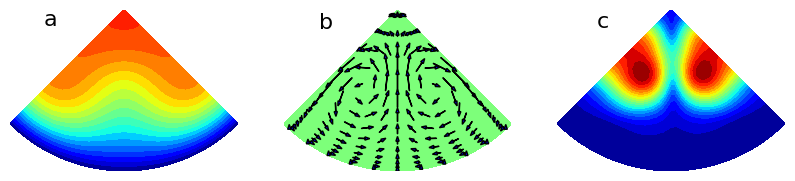
\includegraphics[width=1\linewidth]{pipetw_means.png}}
\center{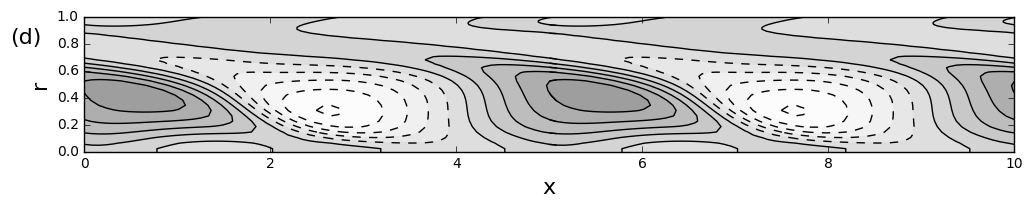
\includegraphics[width=1\linewidth]{pipetw_v1_ls.png}}
\caption{Поле скорости бегущей волны: (a), (b) --- продольная и поперечная компоненты среднего течения $\V_{tw}$, (c) --- амплитуда пульсаций $\v_{n,tw}$, светлый фон соответствует нулевому значению, темный --- наибольшему; (d) --- продольная компонента $\v_{n,tw}$ в сечении $\theta = 0$, сплошные изолинии --- положительные значения, прерывистые --- отрицательные.}
\label{pipetw_pic}
\end{figure}

Хотя найденная бегущая волна повторяет качественные особенности модельного порыва, наблюдаются некоторые количественные отличия. Для сравнения с модельным порывом, на рисунке \ref{pipetw_amp_pic} горизонтальными линиями приведена средняя амплитуда компонент движения бегущей волны. В отличие от модельного порыва, их значение не зависит от продольной координаты. По аналогии с модельным порывом, в среднем течении $\V_{tw}$ выделена двумерная $\V_{2D,tw} = \overline{\V_{tw}}^\theta$ и трехмерная  $\V_{3D,tw} = \V_{tw} - \V_{2D,tw}$ составляющие. Трехмерная составляющая движения разделена на продольную $\V_{S,tw}$ и поперечную $\V_{V,tw}$ компоненты, связанные с полосами и продольными вихрями, соответственно. Качественно соотношение между интенсивностью компонент движения сохраняется, однако в модельном порыве они достигают больших значений. Наибольшее отличие демонстрирует поперечное движение $\V_V$, для бегущей волны его значение более, чем в три раза ниже наибольшего значения, достигаемого в модельном порыве. Это может объясняться тем, что решение на сепаратрисе является равновесным. Равновесная интенсивность продольных вихрей в бегущей волне обусловлена необходимостью преодоления диссипирующего влияния вязкости. В модельном порыве необходима большая интенсивность вихрей для того, чтобы не только поддерживать, но и формировать полосы в попадающем внутрь порыва ламинарном течении. 


\begin{figure}
\center{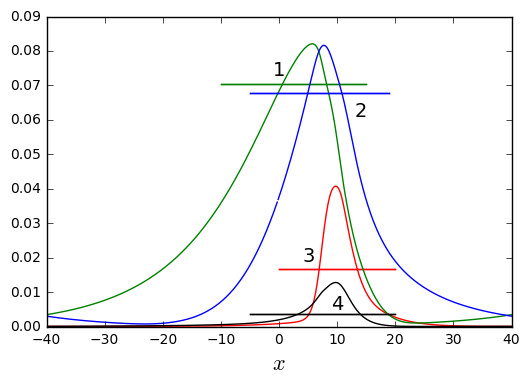
\includegraphics[width=0.5\linewidth]{pipetw_amp.png}}
\caption{Средняя по сечению трубы амплитуда компонент движения бегущей волны (горизонтальные линии) в сравнении с аналогичными величина для модельного порыва (функции переменной $x$): 1 --- движение $\V_S$, ассоциированное с полосами; 2 --- отклонение от течения Пуазейля двумерной компоненты движения $\V_{2D}$; 3 --- пульсационная составляющая движения $\v_n$; 4 --- движение $\V_V$, ассоциированное с продольными вихрями. График повторяет рисунок \ref{amp_pic}.}
\label{pipetw_amp_pic}
\end{figure}

Пульсационная составляющая движения бегущей волны $\v_{n,tw}$ возникает в результате линейной неустойчивости стационарного течения $\V_{tw}$. Наиболее быстро растущее собственное решение линеаризованного уравнения для возмущений \eqref{lin_eq} воспроизводит форму пульсационной составляющей движения и её фазовую скорость. Соответствующий инкремент нарастания $\lambda = 0.0085$. Для сравнения с пульсационной составляющей движения, поле скорости которой представлено на рисунке \ref{pipetw_pic}(c,d), на рисунке \ref{pipetw_lin_pic}(a,b) изображены амплитуда пульсаций, возникающих в линейной задаче, и их мгновенное поле скорости в продольном сечении. Решение линейной задачи имеет более простую форму. Так как среднее течение однородно вдоль трубы и стационарно, линейное решение имеет форму бегущей волны, поле скорости которой меняется по гармоническому закону вдоль трубы и во времени. Как и в случае с модельным порывом, возникающие в рамках линейной задачи пульсации имеют дополнительную симметрию отражения относительно сечения $\theta = \pi/4$, выражаемую уравнением \eqref{dop_sym_eq}. 


\begin{figure}
\center{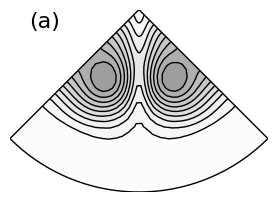
\includegraphics[width=0.33\linewidth]{pipetw_lin_amp.png} 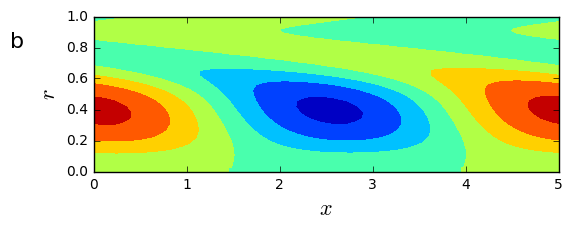
\includegraphics[width=0.6\linewidth]{pipetw_lin_ls.png}}
\caption{Пульсации, возникающее на среднем течении $\V_{tw}$ в рамках линеаризованных уравнений: (a) --- амплитуда пульсаций, светлый фон соответствует нулевому значению, темный --- наибольшему; (b) --- продольная компонента скорости в сечении $\theta = 0$, сплошные изолинии --- положительные значения, прерывистые --- отрицательные. }
\label{pipetw_lin_pic}
\end{figure}

%\lambda = - 0.0065


Возникающая на сепаратрисе бегущая волна, таким образом, воспроизводит основные элементы цикла самоподдержания модельного порыва, но имеет более простую форму. В сопутствующей системе отсчета её поле скорости оказывается стационарным. В потоке выделяются полосы повышенной и пониженной скорости. Области пониженной скорости имеют зигзагообразную форму. В системе отсчета наблюдателя движение представляет собой периодическое смещение области пониженной скорости в угловом направлении. С периодическим движением может быть ассоциирована пульсационная составляющая поля скорости. Было показано, что она возникает в результате линейной неустойчивости среднего течения, воспроизводящего полосчатый профиль скорости. Среднее течение в этом случае однородно вдоль трубы, что объясняет тот факт, что решение имеет форму бегущей волны. Также в потоке могут быть выделены стационарные продольные вихри, ответственные за образование полосчатого профиля скорости, не меняющиеся вдоль трубы. Как будет показано далее, простота поведения бегущей волны позволяет выделить некоторые закономерности движения, справедливые также и для модельного порыва, и продемонстрировать их в строгом виде. В частности, при её анализе был выделен механизм нелинейного взаимодействия пульсаций, поддерживающий существование продольных вихрей. 


\section{Механизм образования продольных вихрей на примере точной бегущей волны}

Принято считать, что продольные вихри, ответственные за образование полос, возникают в результате некоторого нелинейного взаимодействия пульсаций, однако детали такого взаимодействия не установлены. Прояснить процесс формирования продольных вихрей позволяет анализ уравнения, описывающего эволюцию продольной завихренности, полученного применением оператора Ротора к уравнению Навье-Стокса \eqref{NSeq_cf}:
\begin{equation}\label{ox_eq}
\pd{\omega_x}{t} - \nu\Laplace \omega_x =  -  (\v - \c_f, \nabla) \omega_x + (\om, \nabla) v_x.
\end{equation}
Здесь $\om = (\omega_x, \omega_r, \omega_\theta) = \rot \v$ --- вектор завихренности, $\c_f$ --- скорость перемещения системы отсчета. Уравнение для стационарной составляющей продольной завихренности получается после осреднения \eqref{ox_eq} вдоль трубы:
\begin{equation}\label{OX_eq}
\pd{\Omega_x}{t} - \nu\Laplace \Omega_x = - (\V, \nabla) \Omega_x + (\Om, \nabla) V_x - \overline{(\v', \nabla) \omega'_x}^x + \overline{ (\om', \nabla) v'_x }^x.
\end{equation}
Здесь  $\Om=(\Omega_x, \Omega_r, \Omega_\theta)$ и $\om'=(\omega'_x, \omega'_r, \omega'_\theta)$ средняя и пульсационная составляющие вектора завихренности. Отметим, что в силу линейности оператора Ротора и осреднения порядок их применения не влияет на результат:
$$
\Om = \overline{\om}^x = \rot \V,
$$ 
$$
\om' = \om - \Om = \rot \v'.
$$ 
В правой части \eqref{OX_eq} первая пара членов описывает изменение продольной завихренности за счет конвективного переноса и деформации вихревых линий осредненного течения, а вторая пара выражает порождение средней завихренности пульсационным движением. При отсутствии пульсаций продольная завихренность постепенно исчезает под действием вязкости. В рассматриваемом течении система находится в равновесии и стационарная продольная завихренность во времени не меняется. Вязкие диссипация и диффузия компенсируются генерацией завихренности членами в правой части \eqref{OX_eq}.

Для выявления определяющих механизмов генерации средней продольной завихренности удобнее рассмотреть уравнение эволюции квадрата $\Omega_x$, получающееся домножением всех членов \eqref{OX_eq} на $2\Omega_x$. Положительный или отрицательный знак у полученных таким образом выражений в правой части уравнения показывает соответственно положительный или отрицательный вклад этого члена в изменение $\Omega_x^2$, а, следовательно, и в интенсивность поперечного движения. Распределение $\Omega_x^2$ по сечению трубы представлено на рисунке~\ref{OXgen_pic}(a). В большей части сечения трубы средняя продольная завихренность близка к нулю. Области концентрации $\Omega_x$ расположены между полосами повышенной и пониженной скорости вблизи области максимальной амплитуды пульсаций.

\begin{figure}
\center{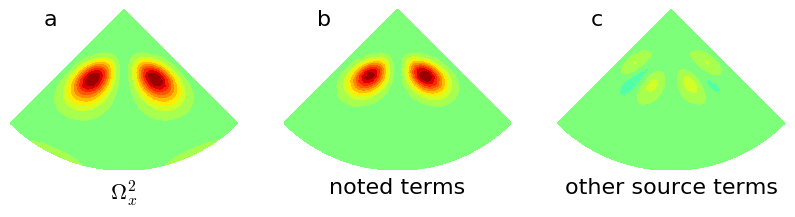
\includegraphics[width=1\linewidth]{pipetw_OXgen.png}}
\caption{Распределение по сечению трубы $\Omega_x^2$ --- (a), вклад в производство $\Omega_x^2$ слагаемых, соответствующих выделенным в \eqref{OXgen_terms} --- (b), вклад остальных слагаемых в правой части \eqref{OX_eq} --- (с), сплошные изолинии соответствуют положительным значениям, прерывистые --- отрицательным.}
\label{OXgen_pic}
\end{figure}

При анализе уравнения \eqref{OX_eq} обнаружено, что два слагаемых в правой части вносят определяющий вклад в производство средней продольной завихренности. Они выделены в уравнении ниже:
\begin{equation}\label{OXgen_terms}
\pd{\Omega_x}{t} = - \overline{v'_x \frac{\d \omega'_x}{\d x}}^x + \overline{ \omega'_x \frac{\d v'_x}{\d x} }^x + ... 
\end{equation}
Соответствующее сумме \eqref{OXgen_terms}  распределение в уравнении для $\Omega_x^2$ представлено на рисунке~\ref{OXgen_pic}(b), а вклад остальных слагаемых правой части \eqref{OX_eq} показан на рисунке~\ref{OXgen_pic}(c). Распределение генерации $\Omega_x^2$ выделенными в \eqref{OXgen_terms} членами практически совпадает по форме с распределением $\Omega_x^2$, тогда как вклад остальных членов не имеет выраженного распределения и на порядок уступает по суммарному вкладу в генерацию $\Omega_x^2$. Таким образом, нет сомнения в том, что стационарные продольные вихри возникают в основном за счет действия выделенной в \eqref{OXgen_terms} пары слагаемых.

Отметим, что пульсации, соответствующие старшей собственной функции линейной задачи об устойчивости среднего стационарного течения, также демонстрируют приведенный выше механизм образования стационарных продольных вихрей. Важно, что это наблюдается только в том случае, когда при анализе устойчивости учитываются как продольная, так и поперечная составляющие среднего течения. Принято считать, что поперечное движение, определяя угловую неоднородность в распределении продольной скорости среднего течения, не может существенным образом влиять на свойства его устойчивости вследствие незначительности своей амплитуды. Поэтому при исследовании линейной устойчивости подобных течений, например, полосчатых структур в турбулентных потоках, наличие поперечного движения обычно не принимается во внимание. В нашем случае пренебрежение поперечным движением приводит к тому, что стационарное течение оказывается линейно устойчивым. Что еще более важно, наименее затухающее возмущение не воспроизводит при этом описанный механизм формирования продольных вихрей. Это связанно с тем, что форма пульсаций продольной завихренности $\omega'_x$ качественно меняется, хотя пульсации продольной скорости $v'_x$ сохраняют свою форму практически неизменной. Тем самым нарушается согласованность  $v'_x$ и $\omega'_x$, необходимая для обеспечения нужного вклада выражения \eqref{OXgen_terms} в производство продольной завихренности.

\begin{figure}
\center{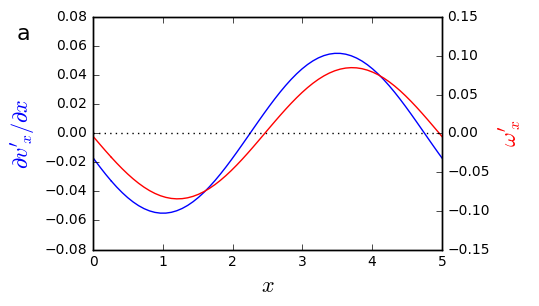
\includegraphics[width=0.5\linewidth]{pipetw_lin_cor.png}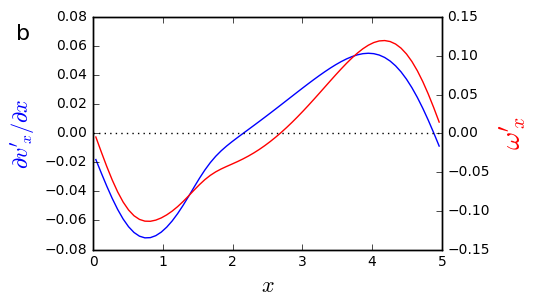
\includegraphics[width=0.5\linewidth]{pipetw_puls_cor.png}}
\caption{Значение $\d v_x' /\d x$ (кривая 1) и $\omega_x'$ (кривая 2) на прямой, проходящей через область, занятую положительным вихрем, при $r = 0.5, \theta = \pi/8$: (a) --- для пульсаций, полученных в линейном приближении; (b) --- для пульсационной составляющей движения бегущей волны. }
\label{OXgen_corr_pic}
\end{figure}


Каждое из двух слагаемых в \eqref{OXgen_terms} дает примерно половину общего вклада в производство средней продольной завихренности. Можно показать, что для пульсаций, полученных в рамках линеаризованной постановки, слагаемые \eqref{OXgen_terms} равны друг другу точно. Среднее поле скорости $\V_{tw}$ однородно вдоль трубы, следовательно, возникающие на нем собственные возмущения меняются вдоль трубы по гармоническом закону. При фиксированных значениях $r$ и $\theta$ пусть  $v'_x = a \sin(\alpha x + \phi)$, $\omega_x' = b \sin(\alpha x + \psi)$, тогда:
\begin{equation} \label{OXgen_iterms_1}
 - v'_x \frac{\d \omega'_x}{\d x} = - \alpha a b \sin(\alpha x + \phi) \cos(\alpha x + \psi),
\end{equation}
\begin{equation} \label{OXgen_iterms_2}
\omega'_x \frac{\d v'_x}{\d x} =  \alpha a b \cos(\alpha x + \phi) \sin(\alpha x + \psi),
\end{equation}
\begin{equation} \label{OXgen_iterms_sum}
 - v'_x \frac{\d \omega'_x}{\d x} + \omega'_x \frac{\d v'_x}{\d x} = \alpha a b \sin(\psi - \phi).
\end{equation}
Осредненные вдоль трубы, слагаемые \eqref{OXgen_iterms_1}, \eqref{OXgen_iterms_2} в точности равны друг другу. Более того, сумма \eqref{OXgen_iterms_sum} не зависит от $x$, что, в частности, позволяет упустить знак осреднения вдоль трубы. Эффективность производства  $\Omega_x$ определяется разностью фаз $\psi - \phi$. В области положительного вихря, при $a,b > 0$, наибольшую эффективность как первому, так и второму слагаемому обеспечивает значение $\psi - \phi = \pi/2$. В этом случае $\d \omega'_x/\d x$ и $v'_x$ положительно коррелированы, в то время как $\d v'_x/\d x$ и $\omega'_x$ --- отрицательно. В области отрицательного вихря ситуация меняется на противоположную. Расчет соответствующих коэффициентов корреляции показывает, что они близки к $\pm1$ в соответствующих областях. В качестве подтверждения на рисунке \ref{OXgen_corr_pic}(a) представлены значения $\d v'_x/\d x$ и $\omega'_x$ на прямой, проходящей через область, занятую положительным вихрем, $r = 0.5, \theta = \pi/8$. Фазы выделенных компонент движения практически совпадают. Указанное свойство сохраняется также для пульсационной составляющей движения $\v_{n,tw}$, для которой аналогичные величины изображены на рисунке \ref{OXgen_corr_pic}(b). Объяснить наблюдаемую согласованность фаз позволяет механизм образования пульсаций продольной завихренности, выделенный при исследовании бегущей волны, представленный в следующем разделе. Отметим, что, так как решения являются бегущими волнами, изображенная на рисунке \ref{OXgen_corr_pic} картина течения сохраняется неизменной во времени. 


\section{Механизм образования пульсаций продольной завихренности на примере точной бегущей волны}

Для выявления механизма формирования выделенной связи между пульсациями продольных компонент скорости и завихренности рассмотрим уравнение эволюции $\omega'_x$, получающееся вычитанием \eqref{OX_eq} из \eqref{ox_eq}:
\begin{multline}\label{ox1_eq}
\pd{\omega'_x}{t} - \nu \nabla^2 \omega'_x = - (\V - \c_f, \nabla) \omega'_x - (\v', \nabla) \Omega_x
+(\Om, \nabla) v'_x + (\om', \nabla) V_x -\\- (\v', \nabla) \omega'_x  + (\om', \nabla) v'_x  + \overline{(\v', \nabla) \omega'_x)}^x  - \overline{(\om', \nabla)}^x.
\end{multline}
Удобнее работать с уравнением, описывающим изменение среднего квадрата пульсаций продольной завихренности $\overline{\omega'_x\omega'_x}^x$, получающимся умножением каждого из слагаемых в \eqref{ox1_eq} на~$2\omega'_x$ c последующим осреднением вдоль трубы. Слагаемые в этом уравнении не зависят от времени и продольной координаты, сумма слагаемых в правой части балансируется вязким членом в левой части. Как и в предыдущем случае, в правой части уравнения удается выделить существенные слагаемые, ответственные за возникновение пульсаций~$\omega'_x$.


Распределение $\overline{\omega'_x \omega'_x}^x$ по сечению трубы изображено на рисунке~\ref{ox1gen_pic}(a). Основные пульсации $\omega'_x$ наблюдаются в центре расчетной области около оси трубы. На месте расположения продольных вихрей также присутствуют пульсации $\omega'_x$, но меньшей интенсивности. В остальной части трубы их амплитуда близка к нулю. Обнаружено, что за генерацию пульсаций $\omega'_x$ в центральной части трубы и на месте продольных вихрей отвечают два разных механизма. Первый дает пульсации большей амплитуды, однако, за возникновение стационарных продольных вихрей ответственны пульсации, производимые вторым механизмом, так как именно они оказываются согласованными с пульсациями $v'_x$ нужным образом.


\begin{figure}
\center{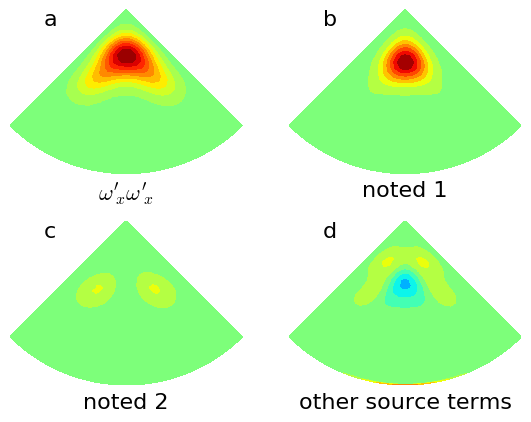
\includegraphics[width=0.66\linewidth]{pipetw_ox1gen.png}}
\caption{Распределение среднего квадрата пульсаций продольной завихренности $\overline{\omega'_x \omega'_x }^x$ в сечении трубы --- (а) и вклад в его производство со стороны слагаемых \eqref{ox1gen_add_terms} --- (b), слагаемого \eqref{ox1gen_main_terms} --- (c) и суммы остальных слагаемых правой части \eqref{ox1_eq} --- (d); сплошные изолинии --- положительные значения, прерывистые --- отрицательные.}
\label{ox1gen_pic}
\end{figure}


Первый механизм формирования~$\omega'_x$ связан с наличием нормальных к стенке вихрей в пульсационной составляющей движения. Можно провести аналогию между неустойчивостью, возникающей на полосе замедления, и неустойчивостью в следе за телом. Пульсационная составляющая движения напоминает дорожку Кармана. В ней можно выделить последовательность нормальных к стенке вихрей чередующегося знака, двигающихся вниз по полосе пониженной скорости. Им соответствуют области повышенной амплитуды пульсаций радиальной завихренности~$\omega'_r$. На рисунке \ref{pipetw_or1_pic} изображена~$\omega'_r$ в сечении $r = 0.5$, нормальном к выделенной компоненте завихренности. Приведенные на \ref{pipetw_or1_pic}(a) значения посчитаны по пульсациям, полученным в рамках линеаризованной задачи. Аналогичные значения для пульсационной составляющей движения $\v_{n,tw}$ представлены на рисунке \ref{pipetw_or1_pic}(b). Амплитуда~$\omega'_x$ оказывается на порядок ниже амплитуды~$\omega'_r$, амплитуда~$\omega'_\theta$ в центральной части трубы равна нулю в силу симметрии. Таким образом, в центральной части трубы поле завихренности представлено в первую очередь радиальной компонентой и соответствует нормальным к стенке вихрям.

Пульсации продольной завихренности $\omega'_x$ возникают вследствие поворота нормальных к стенке вихрей, происходящего в присутствии градиента продольной скорости $\d V_x/ \d r$, возникающего между полосой замедления и осью трубы. Кроме того, наличие радиального градиента $\d V_x/ \d r$ связано с наличием угловой завихренности $\Omega_\theta = \d V_r / \d x - \d V_x / \d r$. Радиальная пульсационная завихренность $\omega'_r = \d v'_x / r \d \theta - \d v'_\theta / \d x$ за счет первого из слагаемых поворачивает стационарные угловые вихри так, что те также приобретают пульсационную продольную составляющую. В уравнении \eqref{ox1_eq} за описанный механизм отвечают слагаемые:
\begin{equation}\label{ox1gen_add_terms}
\frac{\d \omega'_x}{\d t} = \omega'_r \frac {\d V_x}{\d r} + \frac{\Omega_\theta}{r} \frac{\d v'_x}{\d \theta} + ...
\end{equation}
Несмотря на то, что выделенные в \eqref{ox1gen_add_terms} слагаемые имеют противоположные знаки и в значительной степени компенсируют друг друга при сложении, их вклад в производство $\omega'_x$ значителен (смотри рисунок~\ref{ox1gen_pic}(b)). Они определяют форму пульсаций $\omega'_x$ в области между полосой замедления и осью трубы, где пульсации $\omega'_x$ достигают наибольшего значения. Эти пульсации, однако, практически не участвуют в образовании стационарной составляющей продольной завихренности. Это объясняется тем, что колебания $\omega'_x$, рождающиеся в результате описанного механизма, близки по фазе к колебаниям $v'_x$, так что каждое из слагаемых в выражении \eqref{OXgen_terms} при осреднении дает близкое к нулю значение.

\begin{figure}
\center{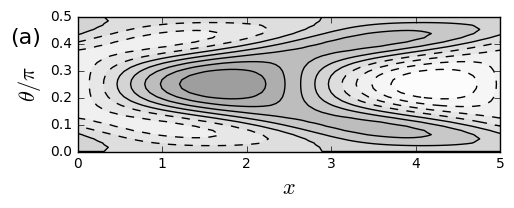
\includegraphics[width=0.45\linewidth]{pipetw_or1_lin.png} 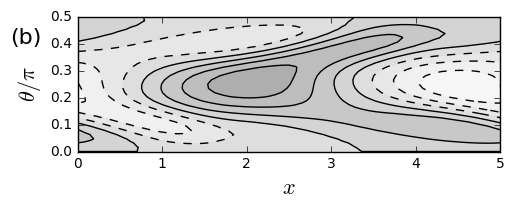
\includegraphics[width=0.45\linewidth]{pipetw_or1.png}}
\caption{Нормальная к стенке компонента завихренности $\omega_r'$ в сечении $r = 0.5$: (а) --- для пульсаций, полученных в рамках линейного приближения; (b) --- для пульсационной составляющей движения бегущей волны. }
\label{pipetw_or1_pic}
\end{figure}

Второй механизм образования пульсаций продольной завихренности $\omega'_x$ связан с перераспределением уже существующей стационарной продольной завихренности $\Omega_x$ за счет пульсационной составляющей продольной скорости $v'_x$ (эффект сжатия/растяжения вихревых линий). В уравнении \eqref{ox1_eq} за описываемый механизм отвечает слагаемое
\begin{equation}\label{ox1gen_main_terms}
\frac{\d \omega'_x}{\d t} = \Omega_x \frac {\d v'_x}{\d x} + ...
\end{equation}
Выделенное в \eqref{ox1gen_main_terms} слагаемое стремится произвести пульсации $\omega'_x$, пропорциональные $\d v'_x / \d x$, что обеспечивает наибольшую эффективность образования~$\Omega_x$ посредством их нелинейного взаимодействия. Важно, что коэффициентом пропорциональности в \eqref{ox1gen_main_terms} выступает значение средней продольной завихренности, таким образом, механизм включается именно в областях концентрации~$\Omega_x$. При этом производимые пульсации $\omega'_x$ положительно пропорциональны пульсациям  $\d v'_x / \d x$ при $\Omega_x>0$ и отрицательно пропорциональны при $\Omega_x<0$, что обеспечивает максимально возможную эффективность производства средней продольной завихренности нужного знака посредством второго из слагаемых выражения \eqref{OXgen_terms}. Очевидно, что пульсации $-v'_x$ и $\d \omega'_x / \d x$ в этом случае также согласованы нужным образом, так что первое слагаемое \eqref{OXgen_terms} близко по значению ко второму.

На рисунке~\ref{ox1gen_pic}(c) приведен вклад выделенного в \eqref{ox1gen_main_terms} слагаемого в производство $\overline{\omega'_x \omega'_x}^x$. Это слагаемое определяет форму пульсаций в области существования продольных вихрей между полосами повышенной и пониженной скорости. Суммарный вклад других слагаемых правой части \eqref{ox1_eq}, не попавших на рисунки~\ref{ox1gen_pic}(b,c), изображен на рисунке~\ref{ox1gen_pic}(d). Эти слагаемые не имеют существенного значения в процессе генерации $\omega'_x$, их суммарный вклад не превышает нескольких процентов. 

Описанный механизм генерации пульсаций продольной завихренности проявляется в области, где фазовая скорость волны, соответствующей пульсационной составляющей течения, близка по значению к локальной продольной скорости среднего течения. На удалении от точки генерации пульсаций, где фазовая скорость волны существенно отличается от средней скорости, выделенный в \eqref{ox1gen_main_terms} механизм генерации $\omega'_x$ практически не работает. Это объясняется тем, что в системе отсчета, связанной с волной, образующаяся посредством механизма \eqref{ox1gen_main_terms} $\omega'_x$ сносится вдоль трубы средним течением. При этом теряется согласованность фаз между $\d v'_x / \d x$ и $\omega'_x$, что делает её рост невозможным. 

Описанный механизм генерации пульсаций продольной завихренности объясняет необходимость учета поперечного движения при исследовании устойчивости стационарного течения. Пренебрежение связанной с поперечным движением $\Omega_x$ делает невозможным генерацию $\omega'_x$ в форме, необходимой для сохранения поперечного движения, а следовательно и всего процесса самоподдержания пульсаций.


\section{Механизм генерации продольных вихрей в модельном порыве}

Выделенный при изучении бегущей волны, возникающей в непротяженной расчетной области, механизм образования продольных вихрей может быть обобщен на модельный порыв. В этом случае разделение движения на среднюю и пульсационную составляющие выполняется путем осреднения по времени в системе отсчета, связанной с порывом. Для точной бегущей волны такое осреднение эквивалентно осреднению вдоль трубы. Осреднение по времени позволяет получить те же результаты для точной бегущей волны, и близкие результаты для бегущей волны, выделяемой в модельном порыве. 

Разделим поле скорости модельного порыва $\v_{mp}$ на среднюю $\V_{mp} = \overline{\v_{mp}}^t$ и пульсационную $\v'_{mp} = \v_{mp} - \V_{mp}$ составляющие (<<mp>> --- <<model puff>>). Соответственно, завихренность стационарной и пульсационной составляющих движения обозначим $\Om_{mp} = \rot \V_{mp}$ и $\om'_{mp} = \rot \v'_{mp}$. Отметим, что завихренность стационарной составляющей движения равна стационарной составляющей поля завихренности: $\Om = \overline{\om}^t$, где $\om = \rot \v$ --- поле завихренности. Аналогично, завихренность пульсационной составляющей движения равна пульсационной составляющей поля завихренности: $\om' = \om - \Om$. 

Как и в случае бегущей волны, стационарная составляющая поля скорости модельного порыва воспроизводит продольные вихри (смотри рисунок \ref{VEL_cs_pic}). В расчетную область попадает пара таких вихрей. Они ответственны за образование полос повышенной и пониженной скорости. Для того, чтобы установить механизм образования продольных вихрей, обратимся к уравнению, описывающему изменение продольной завихренности \eqref{ox_eq}. Его осреднение по времени позволяет получить уравнение баланса стационарной составляющей продольной завихренности $\Omega_x$, имеющее в данном случае вид:
\begin{equation} \label{time_OX_eq}
\pd{\Omega_x}{t} - \nu\nabla^2 \Omega_x = - (\V - \c_f, \nabla) \Omega_x + (\Om, \nabla) V_x - \overline{(\v', \nabla) \omega'_x}^t + \overline{ (\om', \nabla) v'_x }^t.
\end{equation}
Уравнение \eqref{time_OX_eq} аналогично уравнению \eqref{OX_eq} за тем исключением, что в этом случае осреднение производится по времени. Слагаемые в правой части \eqref{time_OX_eq} можно рассматривать как источники $\Omega_x$. Они <<наполняют>> функцию $\Omega_x$ до тех пор, пока их действие не уравновесит вязкость. Среди них могут быть выделены слагаемые, определяющие форму поля $\Omega_x$, связанные с механизмом его формирования. Удобнее работать с уравнением баланса квадрата стационарной продольной завихренности $\Omega_x^2$, полученным скалярным умножением \eqref{time_OX_eq} на $2\Omega_x$. Положительное или отрицательное значение источниковых членов в этом уравнении говорит о положительном или отрицательном их влиянии на образование $\Omega_x$. 


\begin{figure}[h]
\center{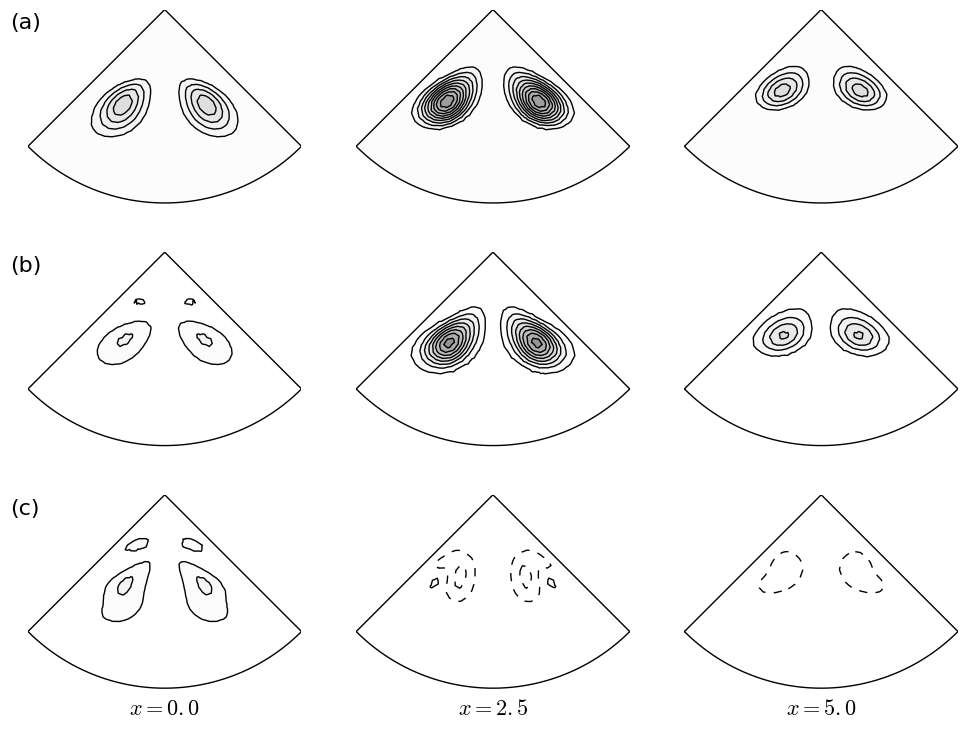
\includegraphics[width=1\linewidth]{puff_OXgen.png}}
\caption{В нескольких сечения трубы приведено значение $\Omega_x^2$ (ряд (а)), а также вклад в образование $\Omega_x^2$ со стороны \eqref{time_OXgen_terms} (ряд (b)) и других слагаемых в правой части уравнения \eqref{time_OX_eq} (ряд (c)). Представлено три сечения из области существования продольных вихрей, $x=0,2.5,5$. Сплошные изолинии соответствуют положительным значениям, прерывистые --- отрицательным.}
\label{mp_OXgen_pic}
\end{figure}

Анализ уравнения \eqref{time_OX_eq} позволил установить механизм образования стационарных продольных вихрей аналогичный выделенному при изучении бегущей волны. За образование продольных вихрей в этом случае ответственна пара слагаемых, сохраненная в уравнении ниже: 
\begin{equation} \label{time_OXgen_terms}
\pd{\Omega_x}{t} = - \overline{v'_x \pd{\omega'_x}{x}}^t + \overline{\omega'_x \pd{v'_x}{x}}^t + ... 
\end{equation}
Слагаемые \eqref{time_OXgen_terms} соответствуют слагаемым \eqref{OXgen_terms}, выделенным при изучении бегущей волны. На рисунке \ref{mp_OXgen_pic} в ряду (а) представлен квадрат продольной завихренности $\Omega_x^2$ в трех сечениях трубы. Его распределение соответствует паре продольных вихрей, расположенных по бокам от полосы замедления (проходящей через центр расчетной области). На рисунке \ref{mp_OXgen_pic} в рядах (b) и (с) в тех же сечения приведен вклад \eqref{time_OXgen_terms} и других слагаемых в правой части уравнения \eqref{time_OX_eq} в образование $\Omega_x^2$. Вклад слагаемых \eqref{time_OXgen_terms} значительно превосходит по величине вклад других слагаемых почти во всех сечениях, он повторяет и определяет форму поля $\Omega_x$. 

\begin{figure}
\center{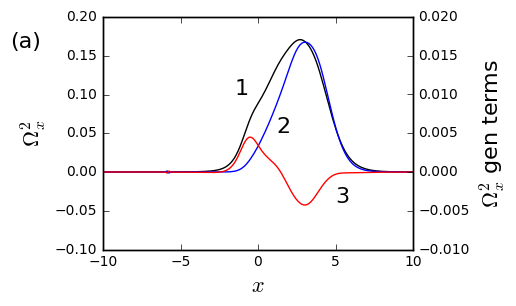
\includegraphics[width=0.5\linewidth]{xline_OXgen.png}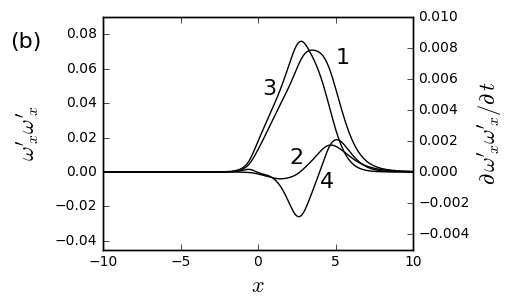
\includegraphics[width=0.5\linewidth]{xline_ox1gen.png}}
\caption{На прямой, проходящей через область, занятую продольным вихрем, при $r = 0.5, \theta = \pi/8$, приведены: (a) --- Квадрат стационарной продольной завихренности (кривая 1), вклад в его производство со стороны \eqref{time_OXgen_terms} (кривая  2) и других слагаемых в правой части уравнения \eqref{time_OX_eq} (кривая 3); (b) --- средний квадрат пульсаций продольной завихренности $\overline{\omega'_x \omega'_x}^t$ (кривая 1) и вклад в его производство со стороны \eqref{time_ox1gen_terms1} (кривая  2), \eqref{time_ox1gen_term2} (кривая  3) и других слагаемых в правой части уравнения \eqref{time_ox1_eq} (кривая  4).}
\label{xline_oxgen_pic}
\end{figure}

На рисунке \ref{xline_oxgen_pic}(a) приведено значение выделенных слагаемых на прямой, проходящей через область, занятую продольным вихрем, $r = 0.5, \theta = \pi/8$. Хотя существует небольшой участок, на котором вклад других слагаемых в правой части уравнения \eqref{time_OX_eq} (изображенный кривой 3) превосходит вклад слагаемых \eqref{time_OXgen_terms} (изображенных кривой 2), выделенные слагаемые определяют форму поля $\Omega_x^2$ (изображенного кривой 1). Таким образом, нет сомнения, что за генерацию стационарных продольных вихрей ответственна выделенная пара слагаемых. Среди слагаемых, представленных кривой 3, можно выделить конвективное слагаемое. Оно переносит $\Omega_x$ вверх по течению, о чем говорит то, что в области $x \approx 3$ оно дает отрицательный вклад, а в области $x \approx 0$ --- положительный. 

В модельном порыве, также как и в бегущей волне, оба слагаемых \eqref{time_OXgen_terms} близки друг к другу по величине. Сохраняется отмеченная в предыдущем разделе согласованность фаз между пульсациями продольной скорости $v'_x$ и продольной завихренности $\omega'_x$, однако форма пульсационной составляющей движения оказывается несколько более сложной. Согласованность фаз объясняется механизмом образования пульсаций продольной завихренности $\omega'_x$, выделенным в модельном порыве, который также совпадает с механизмом, найденным в бегущей волне. 

\begin{figure}[h!]
\center{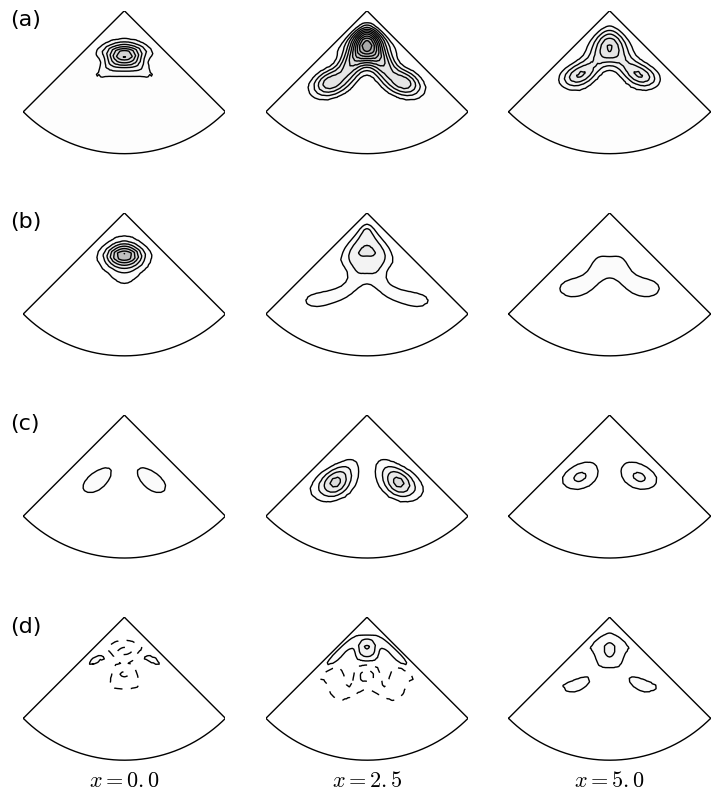
\includegraphics[width=0.9\linewidth]{puff_ox1gen.png}}
\caption{В нескольких сечения трубы изображена интенсивность пульсаций продольной завихренности $\overline{\omega'_x \omega'_x}^t$ (ряд а) и вклад в её генерацию со стороны слагаемых \eqref{time_ox1gen_terms1} (ряд b), слагаемого \eqref{time_ox1gen_term2} (ряд с) и других слагаемых в правой части \eqref{time_ox1_eq} (ряд d). Сплошные изолинии соответствуют положительным значениям, прерывистые --- отрицательным.}
\label{mp_ox1gen_pic}
\end{figure}

Выделить механизм образования пульсаций продольной завихренности $\omega'_x$ позволяет анализ уравнения, описывающего её изменение, полученного по аналогии с \eqref{ox1_eq} вычитанием \eqref{time_OX_eq} из \eqref{ox_eq}:
\begin{multline}\label{time_ox1_eq}
\pd{\omega'_x}{t} - \nu \nabla^2 \omega'_x = - (\V - \c, \nabla) \omega'_x - (\v', \nabla) \Omega_x +(\Om, \nabla) v'_x + (\om', \nabla) V_x - \\ - (\v', \nabla) \omega'_x  + (\om', \nabla) v'_x  + \overline{(\v', \nabla) \omega'_x)}^t  - \overline{(\om', \nabla)}^t
\end{multline}
Удобнее работать с уравнением, определяющим интенсивность пульсаций продольной завихренности $\overline{\omega'_x \omega'_x}^t$, полученным скалярным умножением \eqref{time_ox1_eq} на~$2 \omega'_x$ с последующим осреднением по времени. Анализ этого уравнения позволяет выделить две группы слагаемых, ответственных за образование пульсаций продольной завихренности, имеющих вид:
\begin{equation}\label{time_ox1gen_terms1}
\frac{\d \omega'_x}{\d t} = \omega'_r \frac {\d V_x}{\d r} + \frac{\Omega_\theta}{r} \frac{\d v'_x}{\d \theta} + 
\end{equation}
\begin{equation}\label{time_ox1gen_term2}
+\Omega_x \frac {\d v'_x}{\d x} + ...
\end{equation}
Слагаемые \eqref{time_ox1gen_terms1} отвечают за поворот нормальных к стенке вихрей, возникающих в пульсационной составляющей движения. Приобретая продольную составляющую эти вихри обеспечивают формирование значительных по амплитуде пульсаций $\omega'_x$ в области между полосой замедления и осью трубы. Вклад \eqref{time_ox1gen_terms1} в $\overline{\omega'_x \omega'_x}^t$ представлен на рисунке \ref{mp_ox1gen_pic} в нескольких сечения трубы. Он имеет значительную амплитуду и отвечает за формирование пульсаций $\omega'_x$ в центральной части расчетной области (распределение $\overline{\omega'_x \omega'_x}^t$ представлено на рисунке \ref{mp_ox1gen_pic} в ряду (a)). Однако на месте существования продольных вихрей влияние слагаемых \eqref{time_ox1gen_terms1} невелико. Кроме того, пульсации, формируемые слагаемыми \eqref{time_ox1gen_terms1}, согласованны по фазе с пульсациями $v'_x$ так, что их нелинейное взаимодействие, выраженное слагаемыми \eqref{time_OXgen_terms}, близко к нулю. За образование продольных вихрей ответственно слагаемое \eqref{time_ox1gen_term2}. Его вклад в $\overline{\omega'_x \omega'_x}^t$ представлен на рисунке \ref{mp_ox1gen_pic} в ряду (c). Оно создает пульсации $\omega'_x$ на месте существования продольных вихрей, согласованные с пульсациями $v'_x$ так, что их нелинейное взаимодействие эффективно поддерживает существование продольных вихрей. Другие слагаемые в правой части уравнения \eqref{time_ox1_eq} существенного влияния на интенсивность $\omega'_x$ не оказывают, их вклад в образование $\overline{\omega'_x \omega'_x}^t$ приведен в ряду (d). Можно отметить, что они включают конвективные слагаемые, обеспечивающие перенос существующих пульсаций $\omega'_x$, создаваемых слагаемым \eqref{time_ox1gen_terms1}, вниз по течению. При $x \le 0$ в области между полосой замедления и осью трубы конвективное слагаемое дает отрицательный вклад, а при $x \ge 2$ --- положительный, так как оно переносит $\omega'_x$ из первой области во вторую.

На рисунке \ref{xline_oxgen_pic}(b) приведено значение вклада в формирование $\overline{\omega'_x \omega'_x}^t$ каждой из выделенных групп слагаемых на прямой, проходящей через область, занятую продольным вихрем, $r = 0.5, \theta = \pi/8$. Как только что обсуждалось, подавляющий вклад в образование $\overline{\omega'_x \omega'_x}^t$  дает слагаемое \eqref{time_ox1gen_term2} (кривая~3). Оно определяет интенсивность пульсаций $\omega'_x$ на этой прямой (значение $\overline{\omega'_x \omega'_x}^t$ представлено кривой 1). Другие слагаемые в правой части уравнения (кривые 2, 4) существенного влияния не оказывают. Группа слагаемых, которым соответствует кривая 4, включает конвективное слагаемое, обеспечивающее перенос пульсаций $\omega'_x$ в этой области вниз по течению, в результате чего при $x \approx 3$ это слагаемое дает отрицательный вклад, а при $x \approx 5$ --- положительный. 

В этом разделе было показано, что выделенный при изучении бегущей волны механизм образования продольных вихрей, обеспечивает их формирование также и в модельном порыве. 


\section{Выводы по главе}

В предыдущей главе представлены результаты численного исследования модельного порыва, в котором было составлено представление о его внутренней структуре и механизме самоподдержания колебаний. В подвижной системе отсчета в модельном порыве выделяются стационарные полосы повышенной и пониженной скорости, вытянутые вдоль стенки трубы. Полосы образуются под действием стационарных продольных вихрей, которые формируются в результате нелинейного взаимодействия нестационарных пульсаций, возникающих из-за неустойчивости полосчатого движения. В настоящей главе представлены определяющие элементы нелинейного механизма образования продольных вихрей. Таким образом, определены все элементы цикла самоподдержания колебаний внутри модельного порыва. 

Установлено, что пульсации продольной скорости, возникающие в результате неустойчивости стационарного полосчатого движения, вызывают появление пульсаций продольной завихренности. Пульсации продольной скорости и продольной завихренности оказываются согласованными по фазе таким образом, что их нелинейное взаимодействие усиливает продольные вихри. Продольные вихри формируются на месте возникновения пульсаций, в области между полосами повышенной и пониженной скорости, оказываясь расположенными наиболее удачным образом для поддержания существования этих полос.

Пульсации возникают в результате линейной неустойчивости полосчатого течения и могут быть воспроизведены в рамках линеаризованных уравнений. Решения линейной задачи устойчивости также воспроизводят описанный выше механизм поддержания продольных вихрей, но только в том случае, когда в исследуемом на устойчивость течении учтено не только продольное, но и поперечное движение, индуцируемое этими вихрями. Невзирая на небольшую амплитуду поперечного движения, его учет необходим для адекватного описания пульсаций продольной завихренности. 

Также в главе представлена бегущая волна, возникающая на сепаратрисе в непротяженной расчетной области. Она напоминает бегущую волну, возникающую в передней части порыва, но является точной в том смысле, что её поле скорости меняется вдоль трубы и во времени строго периодическим образом. Простота поведения выделенного решения позволяет на его примере в более простой и в тоже время строгой форме продемонстрировать особенности движения, связанные с самоподдержанием колебаний.

Пример бегущей волны показывает, что механизм поддержания пульсаций в потоке может быть сформулирован и изучен в двумерной постановке в нормальной к основному потоку плоскости. Возникающие на среднем течении пульсации в линейном приближении меняются вдоль трубы по гармоническому закону и могут быть представлены двумерным полем амплитуды и фазы. Их нелинейное взаимодействие определяет форму продольных вихрей, которые также представляются двумерным полем продольной завихренности. Однородные вдоль трубы вихри приводят к образованию полос повышенной и пониженной скорости, также однородных вдоль трубы. 

Можно отметить, что выделенный механизм образования продольных вихрей схож с механизмом линейной неустойчивости. На фоне пульсаций продольной скорости в области их возникновения, где их фазовая скорость близка к скорости жидкости, поле скорости теряет устойчивость к продольным вихрям. Скорость роста стационарной составляющей продольной завихренности пропорциональная амплитуде её пульсаций, а скорость роста амплитуды пульсаций пропорциональна средней составляющей. Аналогичная неустойчивость может иметь место в следе за телом или в слое смешения. 

Полосчатые структуры являются неотъемлемой частью всех сценариев самоподдержания пристенной турбулентности. Можно ожидать, что выделенный механизм генерации продольных вихрей, поддерживающих полосчатые структуры, имеет отношение не только к турбулентным порывам в трубах, но и к более широкому классу пристенных турбулентных течений. 





